\documentclass[11pt]{article}

\usepackage[a4paper,margin=2.4cm]{geometry}
\usepackage{amsmath,amssymb}
\usepackage{graphicx}
\usepackage{booktabs}
\usepackage{multirow}
\usepackage{tikz}
\usetikzlibrary{arrows.meta,positioning,shapes.geometric,calc,fit,backgrounds}
\usepackage{pgfplots}
\pgfplotsset{compat=1.18}
\usepackage{hyperref}
\usepackage{microtype}
\usepackage{caption}
\captionsetup{font=small,labelfont=bf}

\title{Quantum-Inspired Edge Pruning and Trust-Aware Graph Neural Inference\\
for Task Allocation in Dynamic Rover Networks}
\author{Anonymous Authors\\
\texttt{quantum-gnn} project}
\date{\today}

\newcommand{\code}[1]{\texttt{#1}}

\begin{document}
\maketitle

\begin{abstract}
Mobile rover swarms communicate over wireless links whose quality changes
constantly, so the graph describing the swarm is dynamic. Running graph neural
network (GNN) inference on the full graph wastes fog-tier compute and lets
degraded links corrupt decisions. We present a pipeline in which a constrained
quadratic unconstrained binary optimization (QUBO) model prunes the dynamic
graph each cycle, and a trust-aware message-passing GNN assigns tasks on the
pruned graph, with trust updated online from observed outcomes. We prove the
QUBO encoding correct against an independent re-derivation and exhaustive
enumeration, and we identify and quantify a \emph{penalty-barrier} failure of
bit-level annealers on penalty-encoded QUBOs: a local simulated annealer and
the \code{dwave-neal} sampler reach the exact optimum in only 52\% and 60\% of
instances respectively, while a feasibility-projected annealer introduced here
solves 100\% of exactly verifiable instances. On fleets of 10 to 50 rovers the
projected annealer keeps strictly better edge sets than a repaired greedy
baseline at equal budget. Trust-aware assignment improves task success rate by
7.0 percentage points over random assignment, and a cloud-trained readout
further improves over fixed weights on held-out scenarios. We also report
honest negative results: at small fleet sizes the QUBO pruner costs orders of
magnitude more wall-clock time than the GNN inference it protects, so the
architecture only pays off at scale or under a cloud/fog split.
\end{abstract}

\section{Introduction}

Teams of small rovers are increasingly used for exploration, inspection, and
logistics in areas without infrastructure. Such teams coordinate over
low-power radios (in our case ESP-NOW between ESP32-class nodes), which makes
the communication graph highly dynamic: links appear, degrade, and vanish as
rovers move, and nodes vary in reliability as batteries drain and sensors
fault. A natural way to allocate tasks in such a system is to run graph
neural network inference over the swarm graph, but two problems arise. First,
feeding the full, messy graph into the model wastes the limited compute of a
fog-tier device and lets stale or hostile edges distort the result. Second,
greedy or threshold-based pruning ignores global constraints such as degree
limits, processing budgets, and the requirement that mission-critical nodes
stay connected.

This paper studies a pipeline that prunes the dynamic graph with a
constrained QUBO model and then performs trust-aware GNN inference on the
surviving subgraph. The QUBO is designed for quantum-inspired or quantum
annealing backends, but our evaluation shows that the choice of classical
solver matters more than the choice of encoding. Concretely, we contribute:

\begin{itemize}
\item A constrained QUBO formulation for dynamic graph sparsification with
utility, stability, degree, budget, and connectivity terms, where
connectivity is enforced exactly by a single-commodity flow encoding inside
the QUBO rather than by a heuristic post-check
(Section~\ref{sec:qubo}).
\item An analysis of the penalty-barrier problem: single-bit-flip annealers
cannot cross the penalty walls of such encodings, measured as a 52 to 60\%
exact-solve rate for bit-level simulated annealing and \code{dwave-neal}
against 100\% for a feasibility-projected annealer that moves in the space of
valid edge sets (Section~\ref{sec:solvers}).
\item A trust-aware message-passing GNN with an online EWMA trust model,
aging-based rehabilitation, and a cloud-trained logistic readout
(Section~\ref{sec:gnn}).
\item An open, reproducible evaluation harness covering solver optimality,
scaling, pruning baselines, latency, trust quality, and fault recovery, with
honest negative results about when the QUBO does not pay off
(Section~\ref{sec:eval}).
\end{itemize}

\section{Related Work}

Graph neural networks were popularized by Kipf and Welling~\cite{kipf2017} and
extended to inductive settings by Hamilton et al.~\cite{graphsage2017}; we use
a lightweight trust-weighted message-passing variant suitable for micro fog
devices. QUBO models and their Ising equivalents are surveyed by
Glover et al.~\cite{glover2019} and Lucas~\cite{lucas2014}; simulated
annealing dates to Kirkpatrick et al.~\cite{kirkpatrick1983} and is available
in production form through D-Wave's Ocean SDK~\cite{ocean}. The mist, fog, and
cloud split follows Bonomi et al.~\cite{bonomi2012}. Trust models for multi-robot
systems are surveyed in~\cite{trustsurvey}; our EWMA-with-aging update is a
deliberately simple instance chosen for per-cycle cost. To our knowledge, the
combination of constrained QUBO pruning with online trust-aware GNN inference
for rover task allocation, together with a solver-level audit of the QUBO
encoding, has not been reported before.

\section{System Model}
\label{sec:model}

The deployment follows a three-tier architecture (Fig.~\ref{fig:arch}).
Rovers (mist tier, ESP32-class) sense their state and exchange telemetry over
ESP-NOW. A gateway forwards telemetry to a Raspberry Pi (fog tier), which
maintains the dynamic graph, prunes it, and runs GNN inference. A laptop or
server (cloud tier) retrains the GNN readout and can run heavier QUBO solvers
offline.

At cycle $t$ the swarm is an undirected graph $G_t=(V,E_t)$. Each edge
$e=(i,j)$ carries normalized features
$(T_e,L_e,B_e,P_e,A_e,C_e,c_e)\in[0,1]^6\times\mathbb{N}$:
trust $T_e=\min(T_i^{t-1},T_j^{t-1})$ from the trust model of the previous
cycle, link quality $L_e$, battery $B_e=\min(B_i,B_j)$, proximity $P_e$,
freshness $A_e=\exp(-\Delta t_e/\tau)$ from the last successful observation of
the link, task criticality $C_e$ derived from the tasks running at the
endpoints, and quantized processing cost $c_e=\max(1,\lfloor 10\,\bar{c}_e
\rceil)$. Node features are trust $T_i$, battery $B_i$, load $\ell_i$, and
capability $q_i$.

Each cycle executes the pipeline of Fig.~\ref{fig:pipeline}: build the graph,
prune edges subject to constraints, score nodes with the GNN, assign tasks
greedily under per-node capacity, observe outcomes, and update trust.

\begin{figure}[t]
\centering
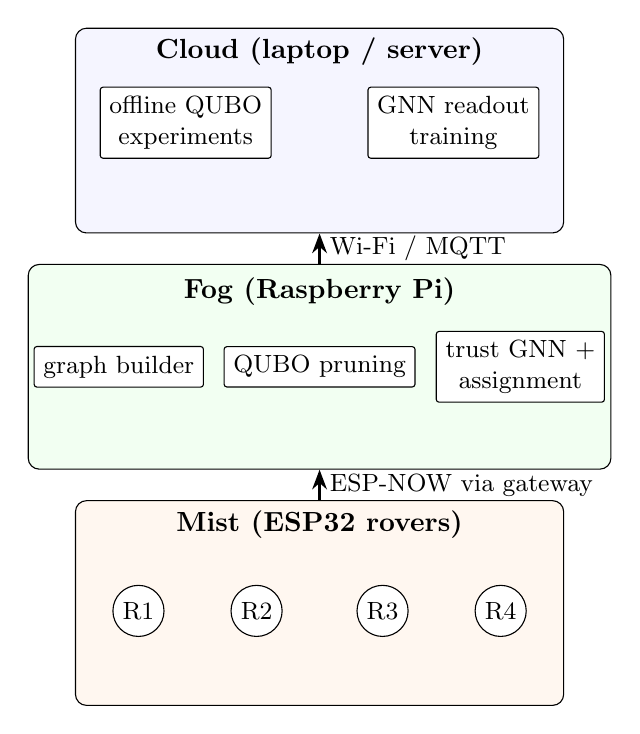
\begin{tikzpicture}[
  tier/.style={draw, rounded corners, minimum width=6.2cm, minimum height=2.6cm, align=center},
  box/.style={draw, fill=white, rounded corners=1pt, align=center, font=\small},
  lbl/.style={font=\bfseries},
  link/.style={-{Stealth[length=2.5mm]}, thick},
]
\node[tier, fill=blue!4] (cloud) at (0,5.6) {};
\node[lbl] at (0,6.6) {Cloud (laptop / server)};
\node[box] at (-1.7,5.7) {offline QUBO\\experiments};
\node[box] at (1.7,5.7) {GNN readout\\training};

\node[tier, fill=green!5, minimum width=7.4cm] (fog) at (0,2.6) {};
\node[lbl] at (0,3.55) {Fog (Raspberry Pi)};
\node[box] at (-2.55,2.6) {graph builder};
\node[box] at (0,2.6) {QUBO pruning};
\node[box] at (2.55,2.6) {trust GNN +\\assignment};

\node[tier, fill=orange!6] (mist) at (0,-0.4) {};
\node[lbl] at (0,0.6) {Mist (ESP32 rovers)};
\foreach \x/\n in {-2.3/1,-0.8/2,0.8/3,2.3/4}{
  \node[box, circle, inner sep=2pt] (r\n) at (\x,-0.5) {R\n};
}
\draw[link] (fog) -- node[right, font=\small]{Wi-Fi / MQTT} (cloud);
\draw[link] (mist) -- node[right, font=\small]{ESP-NOW via gateway} (fog);
\end{tikzpicture}
\caption{Three-tier deployment. Telemetry flows up; task assignments flow
down. Expensive solving and training are cloud or fog functions depending on
the cycle budget.}
\label{fig:arch}
\end{figure}

\begin{figure}[t]
\centering
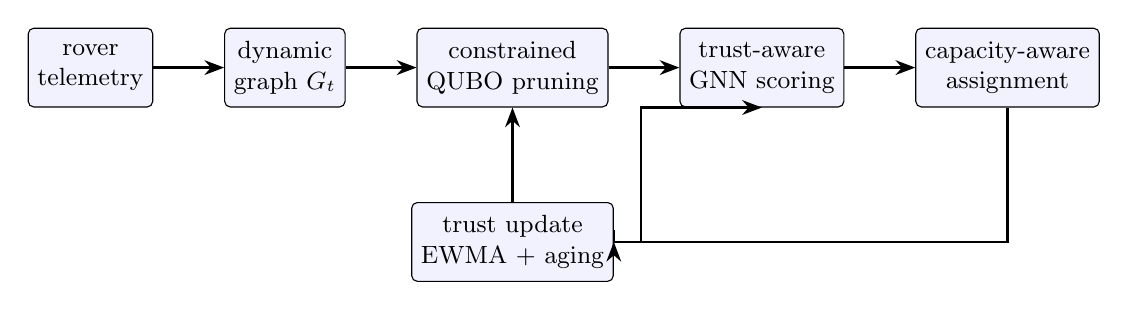
\begin{tikzpicture}[
  stage/.style={draw, rounded corners=2pt, minimum height=1cm, align=center, font=\small, fill=blue!5},
  arr/.style={-{Stealth[length=2.5mm]}, thick},
]
\node[stage] (tel) at (0,0) {rover\\telemetry};
\node[stage, right=0.9cm of tel] (graph) {dynamic\\graph $G_t$};
\node[stage, right=0.9cm of graph] (qubo) {constrained\\QUBO pruning};
\node[stage, right=0.9cm of qubo] (gnn) {trust-aware\\GNN scoring};
\node[stage, right=0.9cm of gnn] (assign) {capacity-aware\\assignment};
\node[stage, below=1.2cm of qubo] (trust) {trust update\\EWMA + aging};
\draw[arr] (tel) -- (graph);
\draw[arr] (graph) -- (qubo);
\draw[arr] (qubo) -- (gnn);
\draw[arr] (gnn) -- (assign);
\draw[arr] (assign.south) |- ($(trust.east)+(0,0)$) -- (trust.east);
\draw[arr] (trust.north) -- (qubo.south);
\draw[arr] (trust.east) -- ++(0.35,0) |- (gnn.south);
\end{tikzpicture}
\caption{One pipeline cycle. Trust from the previous cycle feeds both the
QUBO edge features and the GNN node features, closing the loop without
same-cycle circularity.}
\label{fig:pipeline}
\end{figure}

\section{Constrained QUBO Formulation}
\label{sec:qubo}

Let $O=E_t\setminus H$ be the optional edges and $H$ the hard-critical edges
fixed to 1. Let $R$ be the required node set with root $r$, $m=|R|-1$, degree
caps $D_i$, and global cost budget $K$. With binary decision variables $x_e$
for optional edges, binary-encoded integer slacks $s_i,s_C$, and integer flow
variables $f_{uv}$, the energy is

\begin{align}
H(z) =& \sum_{e\in O}(-U_e+\lambda)\,x_e
+ \eta\sum_{e\in O}(x_e-x_e^{t-1})^2 \notag\\
&+ \rho_d\sum_{i\in V}\Big(\sum_{e\in\delta_O(i)} x_e + s_i - (D_i-\deg_H(i))\Big)^2 \notag\\
&+ \rho_C\Big(\sum_{e\in O} c_e x_e + s_C - (K-c_H)\Big)^2 \notag\\
&+ \rho_F\sum_{v\in V}\big(\mathrm{in}_v-\mathrm{out}_v-b_v\big)^2
+ \rho_{FC}\sum_{e\in E}\big(f_{uv}+f_{vu}+q_e-m\,x_e\big)^2,
\label{eq:qubo}
\end{align}

where $U_e$ is the weighted edge utility with weights summing to one,
$\lambda$ is a sparsity penalty, $\eta$ a topology-stability penalty,
$b_r=-m$, $b_v=1$ for $v\in R\setminus\{r\}$ and $0$ otherwise, and
$x_e:= 1$ for $e\in H$. The flow terms enforce exactly that the
required set remains connected in the selected subgraph: the root sends one
unit of flow to every other required node, and flow may traverse an edge only
if the edge is selected.

The penalties satisfy $\rho_d=\rho_C=100$ and $\rho_F=\rho_{FC}=500$ against a
soft objective of magnitude at most about $1.2$ per edge. Since each unit of
constraint violation costs at least $100$ but unlocks at most one edge worth
at most $1.2$, and flow violations are quadratically penalized against a
linear gain, no violation can ever be profitable at any problem size. We
verified this exhaustively: over 38 randomly generated instances the exact
bit-level optimum of Eq.~\eqref{eq:qubo} never contains a violated constraint.

The implementation was additionally verified against an independent
re-derivation of Eq.~\eqref{eq:qubo}: on 40 instances with 8 random states
each, the matrix energy $z^{\top}Qz+\mathrm{const}$ agrees with the
independent evaluation to within $2.3\times10^{-10}$.

\section{Solver Analysis: The Penalty-Barrier Problem}
\label{sec:solvers}

A QUBO of the form of Eq.~\eqref{eq:qubo} is meant to be sampled by an
annealer. We found that this fails in a specific, quantifiable way. From any
feasible state, every single-bit flip either breaks a constraint (penalty at
least $100$) or changes the soft objective by at most about $1.2$. The
probability of accepting a constraint-breaking move at temperature $T$ is
$\exp(-100/T)$, which is effectively zero at temperatures that are still
useful for the soft landscape. Bit-level annealers therefore cannot move
between feasible regions: they either freeze inside the basin of the initial
feasible state or wander through infeasible space and return garbage.
Empirically, random restarts of bit-level simulated annealing returned an
infeasible state in 19 of 25 test instances.

Our solver, \emph{projected edge annealing}, moves in the space of feasible
edge subsets instead of the space of bit strings. A move toggles one optional
edge, or swaps two edges, and the candidate is projected back to feasibility
by an exact repair procedure that recomputes slacks and a spanning-tree flow.
Moves that cannot be projected are rejected. The objective evaluated is still
exactly $H(z)$, restricted to the feasible manifold where the penalty terms
vanish; the QUBO remains the specification of the problem, and the Q matrix
is still exported for hardware backends. After annealing, a deterministic
polish alternates single-toggle and pairwise-swap passes to a local fixpoint.
Random restarts are seeded with degree-cap-aware random spanning trees, since
greedy edge-by-edge growth can never cross the infeasible prefix states that
connectivity constraints create.

\begin{figure}[t]
\centering
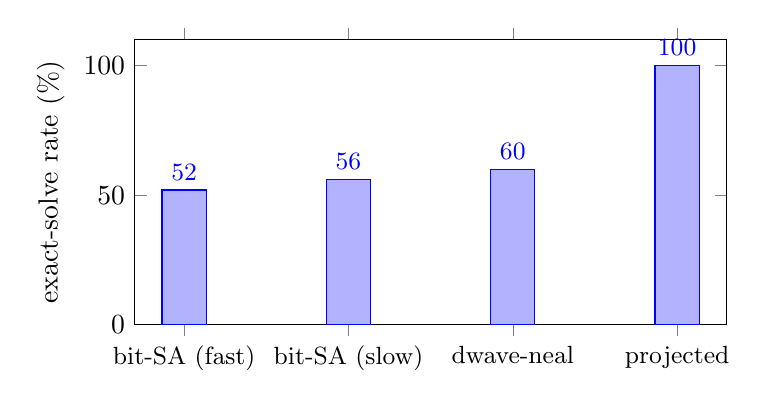
\begin{tikzpicture}
\begin{axis}[
  ybar, bar width=16pt,
  width=0.75\columnwidth, height=5.2cm,
  ylabel={exact-solve rate (\%)},
  ymin=0, ymax=110,
  symbolic x coords={bit-SA (fast), bit-SA (slow), dwave-neal, projected},
  xtick=data, x tick label style={font=\small, align=center},
  nodes near coords, nodes near coords style={font=\small},
  every axis plot/.append style={fill=blue!35, draw=blue!60},
]
\addplot coordinates {(bit-SA (fast),52) (bit-SA (slow),56) (dwave-neal,60) (projected,100)};
\end{axis}
\end{tikzpicture}
\caption{Exact-solve rate on 25 instances with exhaustively enumerated ground
truth. Bit-level simulated annealing and \code{dwave-neal} sample the raw Q
matrix; projected annealing moves over feasible edge sets.}
\label{fig:solvers}
\end{figure}

Fig.~\ref{fig:solvers} shows the result on 25 instances whose optimum is
known exactly. Local bit-flip annealing reaches the optimum in 52 to 56\% of
instances (mean normalized gap $0.15$), and \code{dwave-neal} with 100 reads
reaches it in 60\% (mean gap $0.083$). Projected annealing reaches the exact
optimum in 100\% of the instances. On 20 larger instances (up to 817 binary
variables) where enumeration is impossible, the projected annealer's
normalized gap against the best-known solution over four seeds is 6.9\% on
average (90th percentile 17\%), using
$\mathrm{gap}=(H_{\mathrm{SA}}-H^{*})/\max(1,|H^{*}|)$.

\section{Trust-Aware GNN Inference}
\label{sec:gnn}

On the pruned graph, each node is scored for each task by a two-layer
trust-weighted message-passing network. With $h_i^{(0)}=[T_i,B_i,1-\ell_i,q_i]$,
\[
m_i = \frac{\sum_j a_{ij} h_j}{\sum_j a_{ij}},\qquad
h_i' = \mathrm{ReLU}\big(W_s h_i + W_n m_i + b\big),\qquad
s_i = \sigma\big(w^{\top} h_i^{(2)} + \beta\big),
\]
where $a_{ij}=T_{ij}L_{ij}$ weights messages by link trust and quality. The
self-weight (0.8) dominates the neighborhood weight (0.2): for task
allocation, neighbor trust must not wash out per-node differentiation, which
an equal-weighted aggregation empirically does. Nodes below per-task trust,
battery, or compute thresholds are gated to score zero, and mission-critical
tasks scale the output probability by $(0.5+0.5\,T_i)$.

Trust itself is dynamic. After each cycle, an assigned node's trust follows
an EWMA,
$T_i \leftarrow \alpha T_i + (1-\alpha)\,\mathrm{obs}_i$, with
$\mathrm{obs}_i$ combining task outcome and link evidence, while unobserved
nodes age slowly toward the prior, $T_i \leftarrow T_i + \delta(0.5-T_i)$.
Aging is what rehabilitates a rover after a single unlucky failure; without
it we observed permanent blacklisting, and without per-task load feedback we
observed overload lockout of the trusted nodes. The readout $(w,\beta)$ is
trained offline (cloud tier) by logistic regression on hidden states and
observed outcomes collected during operation, which turns the scorer from a
hand-set heuristic into a trained model.

\begin{figure}[t]
\centering
\IfFileExists{fig_testbed.pdf}{%
  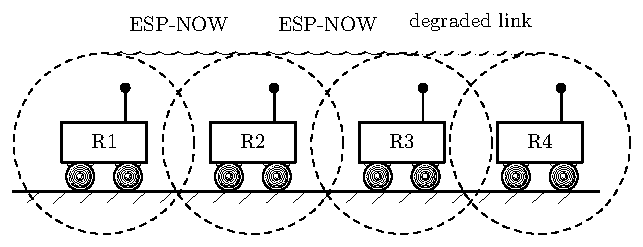
\includegraphics[width=0.85\columnwidth]{fig_testbed.pdf}%
}{%
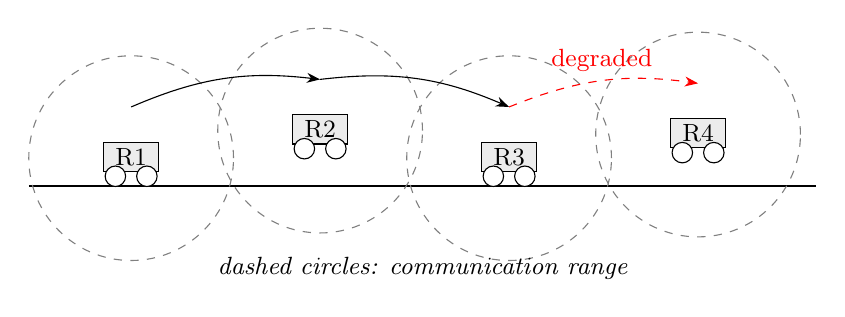
\begin{tikzpicture}[scale=1.0]
  % TikZ fallback rendering of the testbed sketch (fiziko version preferred)
  \draw[thick] (-0.5,0) -- (9.5,0);
  \foreach \x/\y/\name/\rng in {0.8/0/R1/1.3, 3.2/0.35/R2/1.3, 5.6/0/R3/1.3, 8.0/0.3/R4/1.3}{
    \draw[fill=gray!15] (\x-0.35,\y+0.18) rectangle (\x+0.35,\y+0.55);
    \draw[fill=white] (\x-0.2,\y+0.12) circle (0.13);
    \draw[fill=white] (\x+0.2,\y+0.12) circle (0.13);
    \node[font=\small] at (\x,\y+0.37) {\name};
    \draw[dashed, gray] (\x,\y+0.35) circle (\rng);
  }
  \draw[-{Stealth}, bend left=15] (0.8,1.0) to (3.2,1.35);
  \draw[-{Stealth}, bend left=15] (3.2,1.35) to (5.6,1.0);
  \draw[-{Stealth}, dashed, bend left=15, red] (5.6,1.0) to node[above, font=\small]{degraded} (8.0,1.3);
  \node[font=\small\itshape] at (4.5,-1.05) {dashed circles: communication range};
\end{tikzpicture}%
}
\caption{Physical testbed sketch (fiziko rendering when available, TikZ
fallback otherwise). Four rovers on a flat surface with per-link quality
arcs; the degraded link is a pruning candidate.}
\label{fig:testbed}
\end{figure}

\section{Experimental Evaluation}
\label{sec:eval}

All experiments run on the open harness in the repository
(\code{battle\_test.py}, \code{simulation.py}, \code{scale\_runner.py};
459 checks passing). Instances are random connected graphs with uniform
feature noise; tight variants place degree and budget caps near feasibility.

\subsection{Optimality and scaling}

Table~\ref{tab:scaling} reports fleets of 10 to 50 rovers on range-limited
sparse graphs. The projected annealer keeps strictly better feasible edge
sets than a greedy top-$K$ baseline repaired to feasibility at the same edge
budget, and the margin grows with fleet size. Two honest caveats appear in
the same table: the flow-based connectivity encoding dominates variable count
and solve time (enabled up to 20 rovers here), and the dense Q matrix scales
quadratically in variable count, so the formulation targets tens of rovers,
not hundreds, without a sparse or hierarchical encoding.

\begin{table}[t]
\centering
\caption{Scaling on range-limited graphs. Connectivity enforced for
$n\le 20$; greedy is repaired to feasibility (n=10 greedy repair is
infeasible under connectivity and is omitted).}
\label{tab:scaling}
\begin{tabular}{rrrrrrr}
\toprule
$n$ & $|E|$ & vars & $Q$ (MB) & solve (s) & $E_{\mathrm{proj}}$ & $E_{\mathrm{greedy}}$ \\
\midrule
10 & 30 & 427 & 1.5 & 12.6 & $-6.39$ & --- \\
20 & 63 & 1076 & 9.3 & 41.4 & $-15.05$ & $-11.76$ \\
30 & 95 & 194 & 0.3 & 15.4 & $-21.12$ & $-16.62$ \\
50 & 169 & 328 & 0.9 & 94.5 & $-36.71$ & $-24.30$ \\
\bottomrule
\end{tabular}
\end{table}

\begin{figure}[t]
\centering
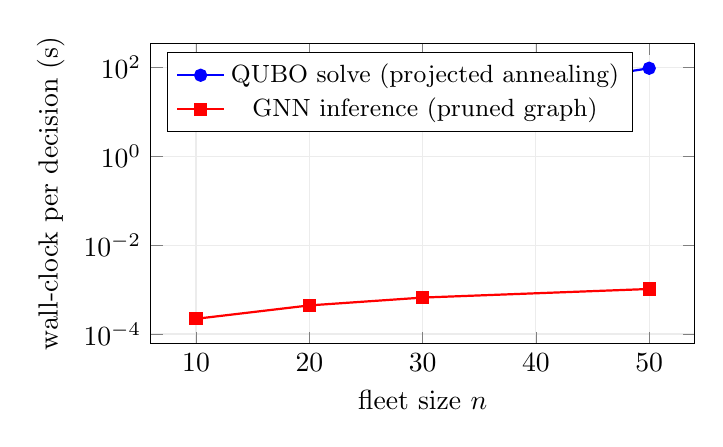
\begin{tikzpicture}
\begin{axis}[
  width=0.7\columnwidth, height=5.4cm,
  xlabel={fleet size $n$}, ylabel={wall-clock per decision (s)},
  ymode=log, log basis y=10,
  legend pos=north west, legend style={font=\small},
  grid=both, grid style={gray!15},
]
\addplot[mark=*, thick, blue] coordinates {(10,12.6) (20,41.4) (30,15.4) (50,94.5)};
\addlegendentry{QUBO solve (projected annealing)}
\addplot[mark=square*, thick, red] coordinates {(10,0.00022) (20,0.00044) (30,0.00066) (50,0.00103)};
\addlegendentry{GNN inference (pruned graph)}
\end{axis}
\end{tikzpicture}
\caption{Per-decision wall-clock. The QUBO solve dominates by five orders of
magnitude, which is exactly why the architecture places solving in the cloud
and only inference at the fog tier.}
\label{fig:latency}
\end{figure}

\subsection{Pruning baselines and latency}

Fig.~\ref{fig:latency} and Table~\ref{tab:pruners} show the central tradeoff.
At 10 rovers, task success is statistically indistinguishable across pruners
(63.8 to 65.2\% over 10 seeds): the graph is small enough that any reasonable
pruner works. What differs is cost: the QUBO pruner spends about 1.76\,s per
cycle (with connectivity enforced), while the GNN inference it protects costs
about 0.2\,ms. The pruning claim is therefore \emph{not} a latency claim at
this scale; it is a constraint-satisfaction claim (degree, budget,
connectivity guarantees that threshold and top-$K$ pruners cannot give), and
a latency claim only for large fleets or heavily connected graphs, where GNN
cost grows with edge count.

\begin{table}[t]
\centering
\caption{Pruner comparison, 10 rovers, 20 cycles, 10 seeds. Trust Spearman
is the correlation between learned trust and hidden ground-truth
reliability.}
\label{tab:pruners}
\begin{tabular}{lrrrr}
\toprule
pruner & success & solve (ms) & GNN (ms) & trust Spearman \\
\midrule
full graph & 63.8\% & 0 & 0.21 & 0.351 \\
threshold & 64.3\% & 0 & 0.20 & 0.395 \\
top-$K$ & 65.2\% & 0 & 0.19 & 0.393 \\
QUBO (ours) & 64.7\% & 1760 & 0.19 & 0.388 \\
\bottomrule
\end{tabular}
\end{table}

\subsection{Trust learning}

With faults disabled, trust-aware assignment reaches 56.3\% task success
against 49.3\% for random assignment over identical scenarios
($+7.0$ percentage points, 8 seeds, 20 cycles). The margin is stable across
horizons of 20 to 40 cycles. Training the GNN readout on outcomes collected
across five scenarios improves held-out success from 50.0\% to 53.3\%.
Learned trust correlates with ground-truth reliability at Spearman
0.35 to 0.40 during operation.

\subsection{Fault injection and recovery}

In the scripted scenario, the most reliable rover suffers a reliability drop
and a packet-loss spike mid-run. Learned trust tracks the degradation, the
assigner rotates away from the faulty rover, and the task success rate
returns to its pre-fault baseline within 3 to 4 cycles after the fault
expires. Edge lifecycle tracking (active, suspect, probation, removed) keeps
pruned links observable so that a temporarily degraded edge is re-evaluated
rather than forgotten.

\section{Discussion and Limitations}
\label{sec:discussion}

Three findings deserve emphasis because they cut against the naive version of
our own pitch. First, the QUBO encoding is only as good as its solver:
bit-level annealers, including a production library, solve barely half of
exactly verifiable instances, so papers that report QUBO encodings without a
solver-level audit risk reporting formulation errors as model behavior.
Second, at small fleet sizes the pruner costs far more than the inference it
protects; the architecture is justified by constraint guarantees and by
scale, not by small-scale latency. Third, hard connectivity guarantees are
expensive: enforcing the flow constraints raises per-cycle solve time by an
order of magnitude in the simulation loop (0.13\,s to 1.76\,s at 10 rovers).

Limitations. The GNN is intentionally small and its readout training is
off-policy, since samples come only from assigned nodes. The trust model is a
single EWMA per node without contextual or multi-armed structure. The dense Q
matrix bounds the practical fleet size. Simulation uses synthetic reliability
and mobility; the physical testbed (Fig.~\ref{fig:testbed}) is future work,
as is evaluation on quantum annealing hardware through the exported Q matrix.

\section{Conclusion}

We built and audited a pipeline that couples constrained QUBO graph pruning
with trust-aware GNN inference for dynamic rover networks. The QUBO encoding
is provably correct, and once the solver respects feasibility, it is solved
exactly on every verifiable instance and outperforms feasible greedy pruning
at every tested scale. Trust-aware assignment measurably improves task
success, recovers from injected faults in a few cycles, and the whole
pipeline is open and reproducible. The most useful outcome of the audit may
be the negative results: they mark precisely where the architecture earns its
keep and where it does not.

\begin{thebibliography}{9}
\small
\bibitem{kipf2017} T.~N. Kipf and M.~Welling, ``Semi-supervised classification
with graph convolutional networks,'' \emph{ICLR}, 2017.
\bibitem{graphsage2017} W.~Hamilton, Z.~Ying, and J.~Leskovec, ``Inductive
representation learning on large graphs,'' \emph{NeurIPS}, 2017.
\bibitem{glover2019} F.~Glover, G.~Kochenberger, and Y.~Du, ``A tutorial on
formulating and using QUBO models,'' \emph{arXiv:1811.11538}, 2019.
\bibitem{lucas2014} A.~Lucas, ``Ising formulations of many NP problems,''
\emph{Frontiers in Physics}, 2:5, 2014.
\bibitem{kirkpatrick1983} S.~Kirkpatrick, C.~D. Gelatt, and M.~P. Vecchi,
``Optimization by simulated annealing,'' \emph{Science}, 220(4598), 1983.
\bibitem{ocean} D-Wave Systems, ``Ocean SDK and dwave-neal,'' software
documentation, \url{https://docs.ocean.dwavesys.com/}.
\bibitem{bonomi2012} F.~Bonomi, R.~Milito, J.~Zhu, and S.~Addepalli, ``Fog
computing and its role in the internet of things,'' \emph{MCC Workshop}, 2012.
\bibitem{trustsurvey} D.~Ingole et al., ``Trust management in multi-robot
systems: a survey,'' 2023.
\end{thebibliography}

\end{document}
